\section{Large language models (LLMS)}

Large language models utilize deep neural networks to generate human-like language output by learning patterns from extensive text data. These models excel at various NLP tasks, including language generation, machine translation, question answering, and sentiment analysis.

The advent of transformer-based architectures, exemplified by GPT (Generative Pre-trained Transformer) and BERT (Bidirectional Encoder Representations from Transformers), marks a recent breakthrough in large language models. These models undergo pre-training on vast datasets, allowing them to learn from massive amounts of data. Subsequently, they can be fine-tuned for specific tasks.

In recent years, large language models like GPT-3 and the more recent GPT-4 have witnessed a significant enhancement in performance and capabilities, achieving remarkable results across a diverse array of benchmarks.

LLMs use various NLP tasks to achieve their goals. For example, tokenization can be
used for pricing the LLM usage when used tokens are counted \cite{openai:tokens}, the models summarize texts, answer questions, etc. Different applications that use NLP are search engines,language translation services, chatbots, text summarization, and question-answering.
While LLMs can incorporate all these tasks and applications, their performance may differ
from those designed for a specific task.

\begin{figure}[H]
    \centering
    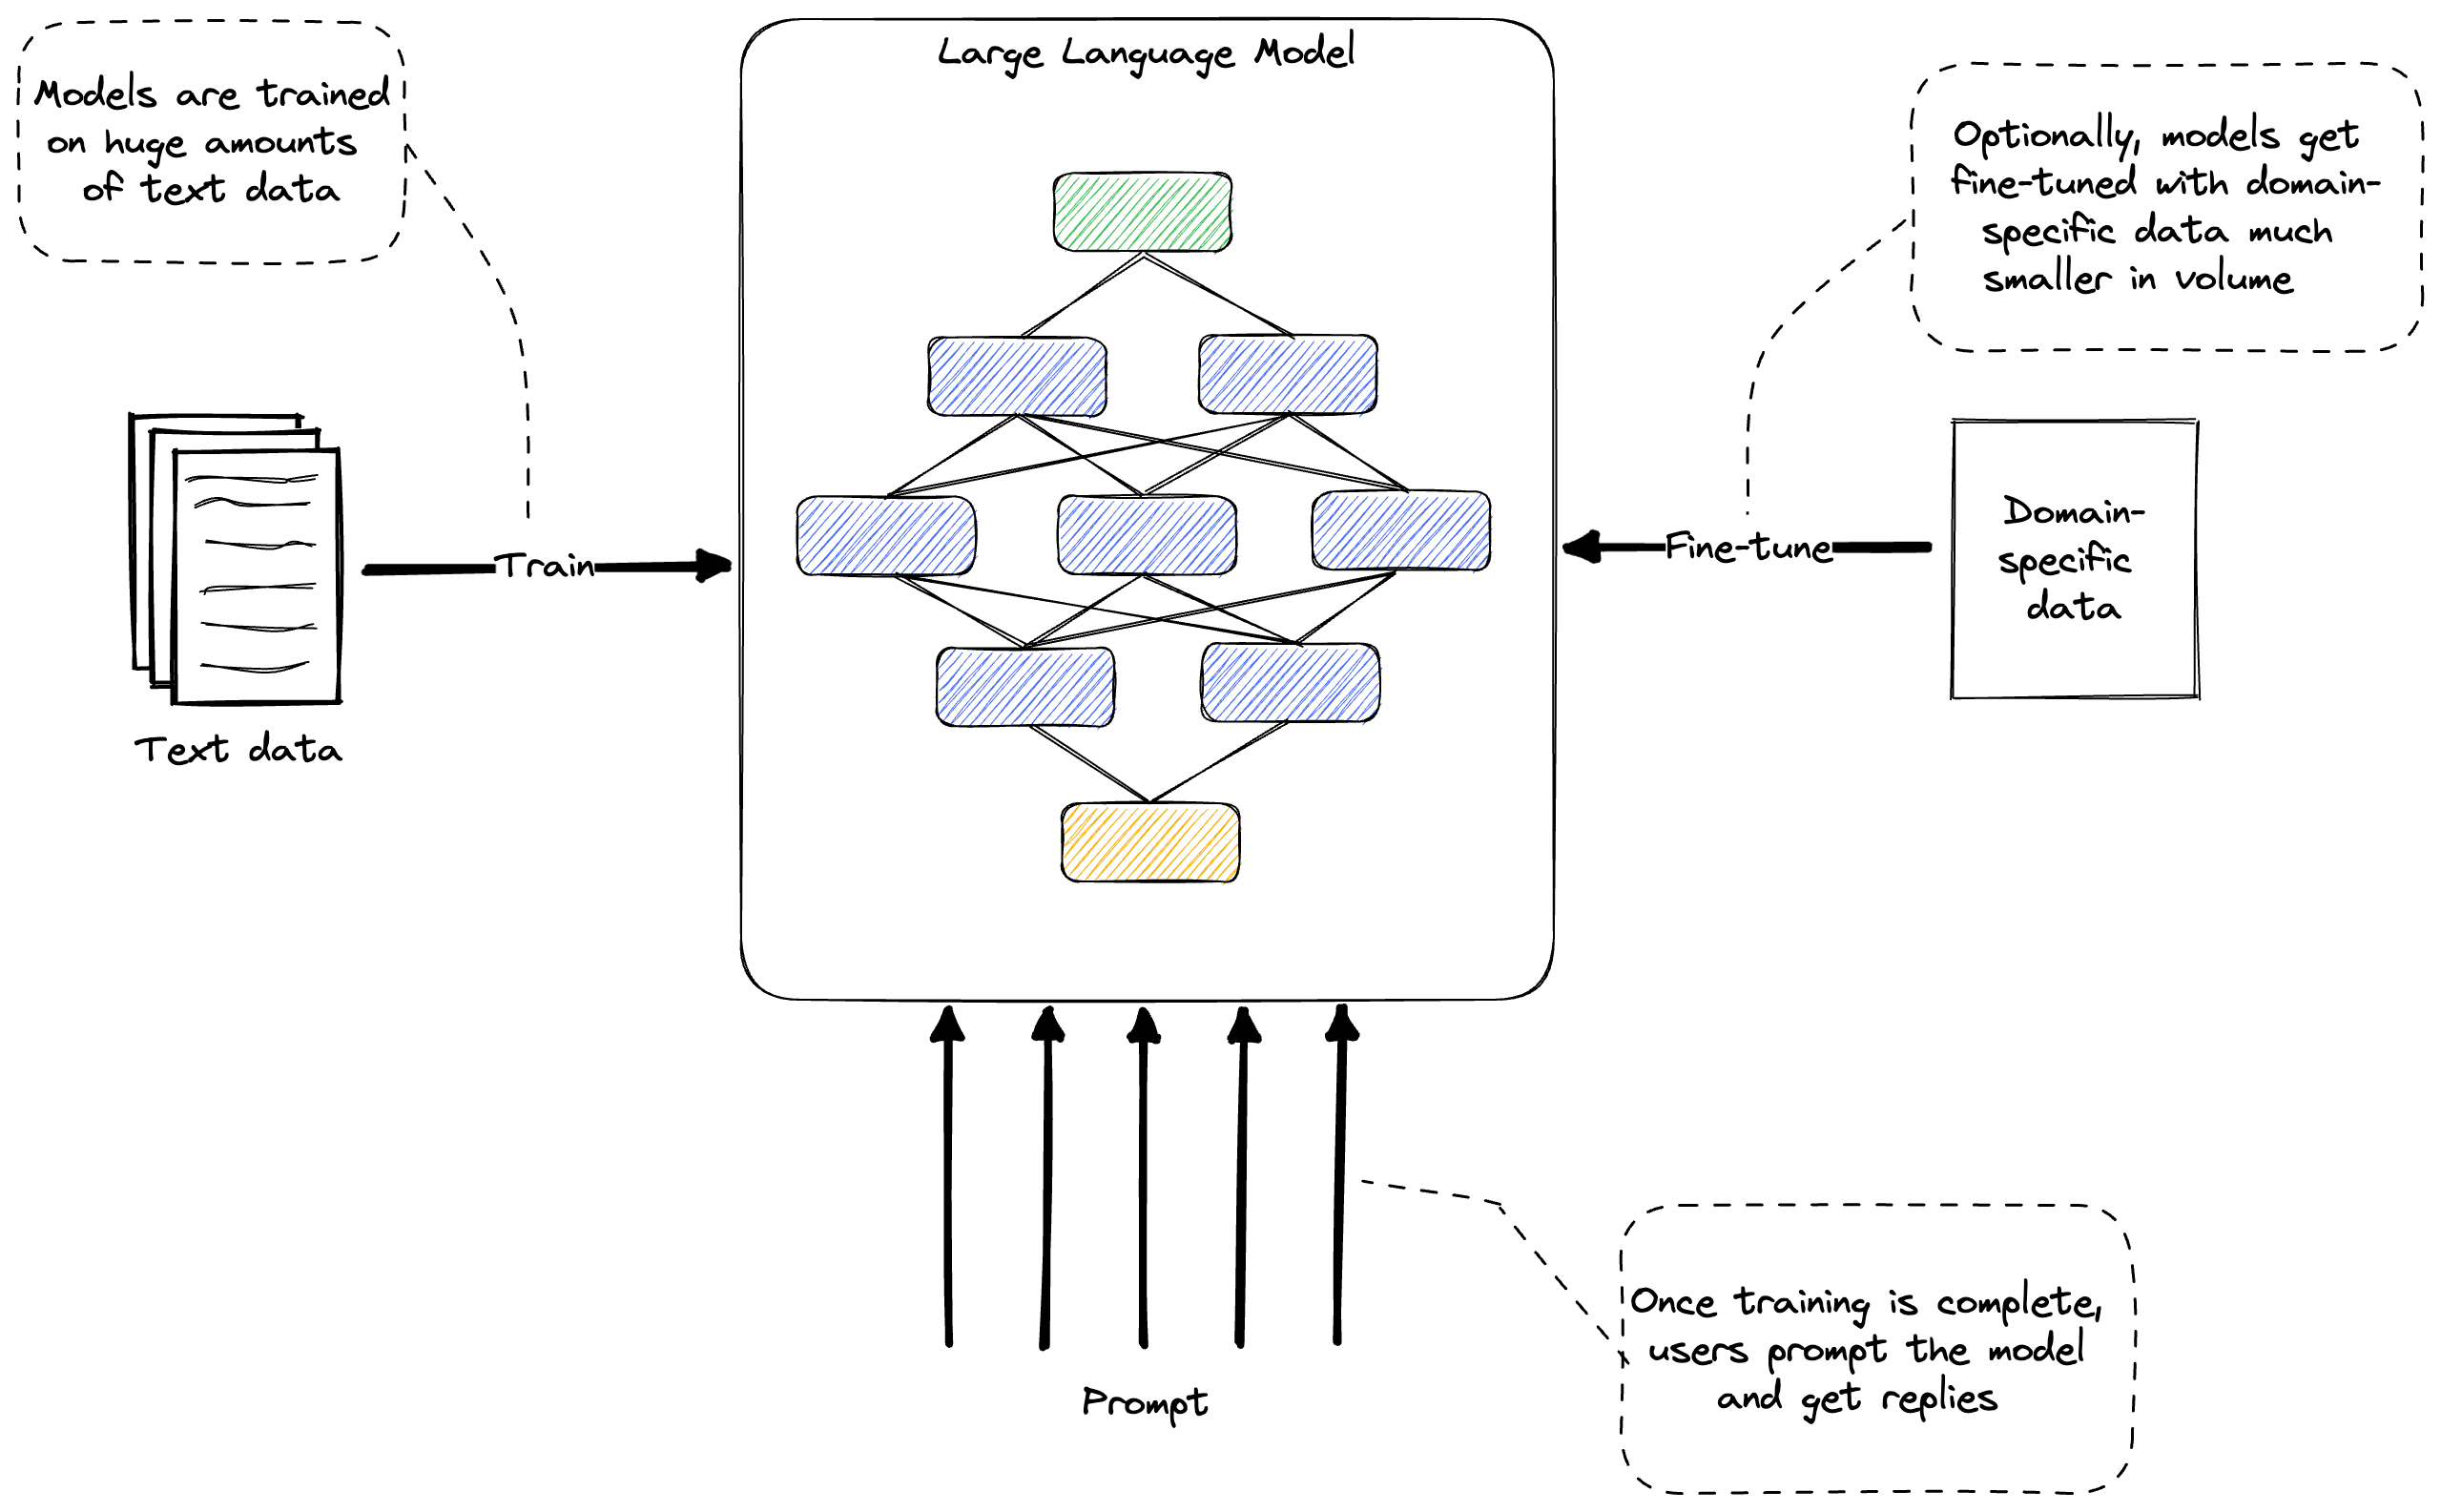
\includegraphics[width=\textwidth,height=6cm,keepaspectratio=true]{llms.png}
    \caption{
        \it{Training, fine tuning, and prompting.}
    }
\end{figure}

\subsection{History of Large Language Models}

Over the years, the development of LLMs has been propelled by advancements in NLP, machine learning, and computing resources. This section offers a comprehensive overview of the significant milestones and breakthroughs that have shaped the evolution of LLMs.

\subsubsection*{Pre-Transformer Era}

\begin{enumerate}
    \item \textbf{Eliza (1964-1966):} One of the earliest NLP programs, Eliza was a simple chatbot developed by Joseph Weizenbaum, designed to mimic a Rogerian psychotherapist. It used pattern matching and substitution to generate responses, laying the foundation for future conversational AI systems.
    \item \textbf{Statistical language models (1980s-2000s):} Statistical language models, such as n-grams, were developed to predict the probability of a word in a sequence based on the preceding words. These models were widely used in tasks like speech recognition and machine translation but struggled with capturing long-range dependencies in text.
    \item \textbf{Neural language models (2003-2013):} Neural language models, such as feedforward and recurrent neural networks (RNNs), emerged as an alternative to statistical models. Bengio et al. (2003) introduced a feedforward neural network for language modeling, while Mikolov et al. (2010) popularized RNN-based models with the release of the RNNLM toolkit.
    \item \textbf{Long Short-Term Memory (LSTM) models (1997-2014):} Hochreiter and Schmidhuber (1997) introduced LSTMs as a solution to the vanishing gradient problem faced by RNNs. LSTMs were later used in sequence-to-sequence models for tasks like machine translation (Sutskever et al., 2014) and formed the basis for several LLMs.
\end{enumerate}

\subsubsection*{Transformer Era}

\begin{enumerate}
    \item \textbf{Attention is All You Need (2017) \cite{vaswani2023attention}:} Vaswani et al. introduced the transformer architecture, which replaced the recurrent layers in traditional models with self-attention mechanisms. This breakthrough enabled the development of more powerful and efficient LLMs, laying the foundation for GPT, BERT, and T5.
    \item \textbf{GPT (2018) \cite{openai:gpt}:} OpenAI released the Generative Pre-trained Transformer (GPT), a unidirectional transformer model pre-trained on a large corpus of text. GPT showcased impressive language generation capabilities and marked the beginning of a new era of LLMs.
    \item \textbf{BERT (2018) \cite{devlin2019bert}:} Google introduced the Bidirectional Encoder Representations from Transformers (BERT) model, which used a masked language modeling objective to enable bidirectional context representation. BERT achieved state-of-the-art performance on numerous NLP tasks, revolutionizing the field.
    \item \textbf{GPT-2 (2019) \cite{radford2019language}} OpenAI released GPT-2, a significantly larger and more powerful version of the original GPT. GPT-2 demonstrated impressive text generation capabilities, generating coherent and contextually relevant text with minimal prompting.
    \item \textbf{T5 (2019) \cite{raffel2023exploring}:} Google's Text-to-Text Transfer Transformer (T5) adopted a unified text-to-text framework for pre-training and fine-tuning, allowing it to be used for various NLP tasks by simply rephrasing the input and output as text. T5 demonstrated state-of-the-art performance across multiple benchmarks.
    \item \textbf{GPT-3 (2020) \cite{brown2020language}:} OpenAI unveiled GPT-3, an even larger and more advanced version of the GPT series, with 175 billion parameters. GPT-3's performance on various NLP tasks with minimal fine-tuning raised questions about the capabilities and potential risks associated with LLMs.
\end{enumerate}

The history of large language models is marked by continuous innovation and progress in the field of natural language processing. As we move forward, LLMs are expected to grow in size, capability, and efficiency, enabling more complex and human-like language understanding and generation. However, the development of these models also brings forth ethical and practical challenges that must be addressed, such as biases, misuse, and computational resource requirements. It is essential for researchers and practitioners to balance the potential benefits of LLMs with their limitations and risks, fostering responsible development and use of these powerful tools.